% note - here expand on EC2, RDS, cache, NoSQL, NAT computing specifications
\section{AWS Services Hardware Specfication \& Cost Estimation}

\begin{figure}[h!]
  \centering
  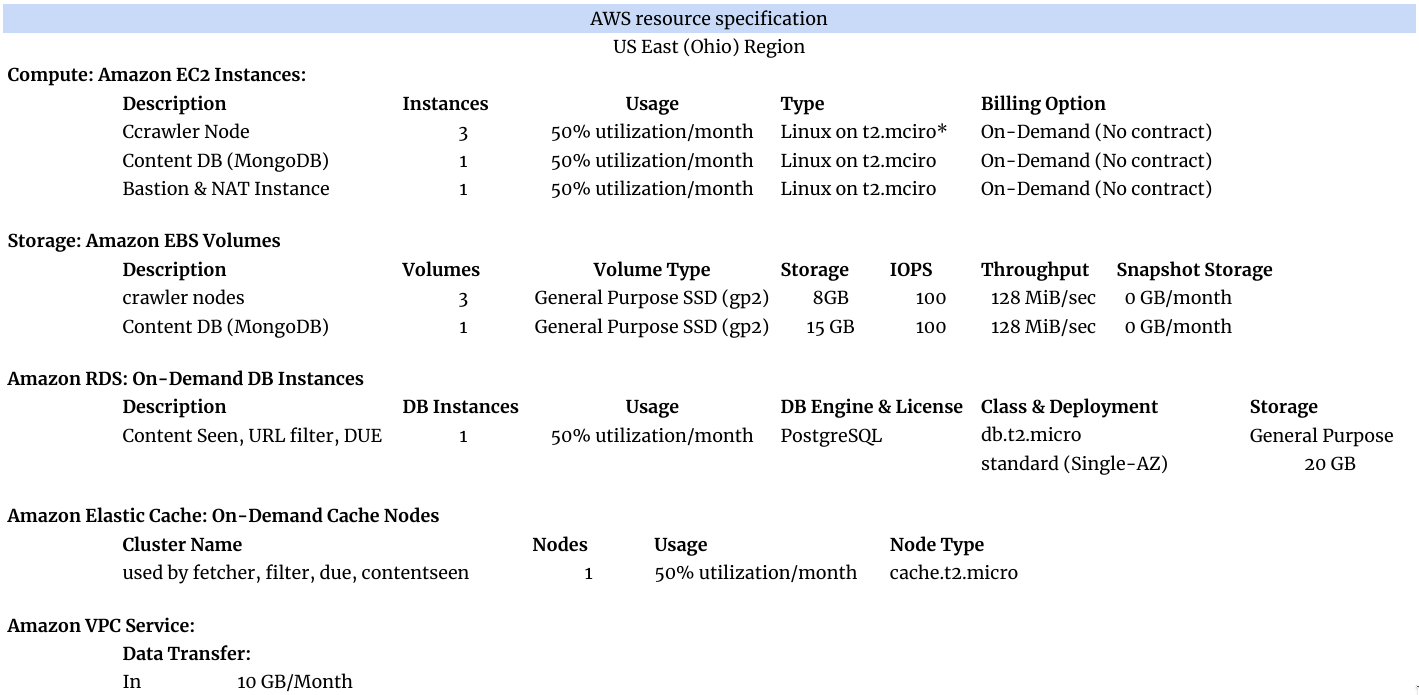
\includegraphics[width=16cm,height=13cm,keepaspectratio]{../media/crawler/aws-resource.png}
  \caption{Whirlpool Hardware Specification on AWS}
  \label{fig:awsspec}
\end{figure}

\noindent
From table \ref{fig:awsspec} under Amazon EC2 services, crawler nodes and the Bastion host sits on a on-demand EC2 instance which is of type t2.micro. The t2.micro has single core virtual CPU (vCPU) with 1 GiB of Memory. Each crawler node runs a message broker - RabbitMQ to interconnect the crawler subsystems. According to RabbitMQ Documentation \cite{rabbitmq}, the host should have at least 128 MB memory available at all times. Moreover,
it wont accept any new messages when it detects that its using more than 40\% of avialable memory. Being
said that, there is always an option to change the current instance type from t2.micro to t2.small and so
on depending on usage. MongoDB which collects extracted text is also hosted on On-Demand t2.micro instance
type, which is a 1 GB, dual-core vCPU operating at 50\% of its capacity.
\\
\\
\noindent
Coming to Amazon Storage,  the crawler node is coupled with Elastic Block Storage(EBS) volume of 8 GiB.
The volume is general purpose SSD capped at 100 IOPS giving a throughput of 128 MB/sec. For mongoDB an
EBS volume of 15GB is used. It is formatted with XFS filesystem for its data directory as recommended in
its production checklist.
\\
\\
\noindent
Whirlpool uses one On-Demand RDS instance with PostgreSQL engine operating at 50\% utilization monthly. The underline managed Operating System is a db.t2.micro deployed in a single AZ. PostgreSQL to store fingerprints of a web page content at a given URL, robots.txt attributes of each site, and URLs already enqueued to be crawled.
\\
\\
Amazon ElasticCache provides a choice between Memcached \& Redis Instance. It will be used by URL filter
subsystem of whirlpool.

\pagebreak

\noindent
Table \ref{fig:awscost} provides approximate monthly billing information of AWS services used by this project to build, test, and run experiments. The calculation was performed using AWS monthly calculator. At the time of this writing, the author is enrolled is 12-month AWS Free tier access which discounts most of the services
the crawler system leverages.

\begin{figure}[h!]
  \centering
  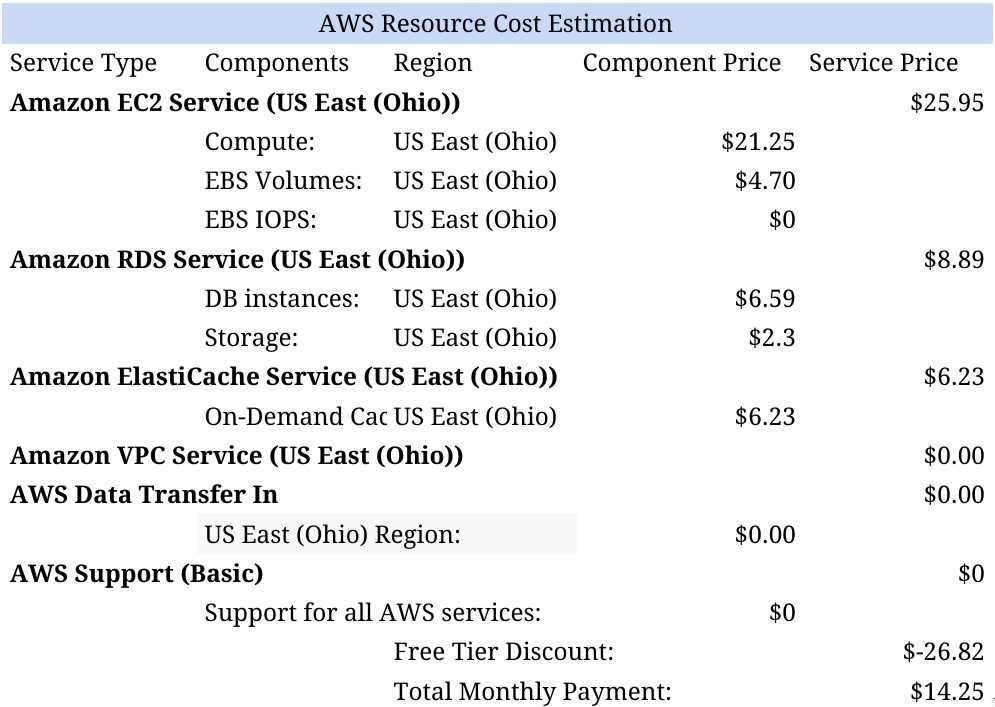
\includegraphics[width=12cm,height=8cm,keepaspectratio]{../media/crawler/aws-resource-cost-estimation.png}
  \caption{Whirlpool Hardware Cost Estimation on AWS}
  \label{fig:awscost}
\end{figure}

\noindent
With the free-tier in use, the total price is dropped almost by 50 \%. Under free tier, EC2 is limited to 750 hours/month which equates to approx. 24 hours/day for 30 days using only Linux, RHEL. Any combination of EBS (SSD/Magnetic) is 30 GiB. Amazon RDS again limited to 750 hours/month upto 20GB of general purpose SSD database
storage. Amazon ElasticCache - 750 hours. NAT instance is priced similar to other EC2 crawler instance types. There is no charge for data transfer between cross-region multi-AZ as this implementation is only us-east-2 single AZ. Also, the data transfer into AWS cloud is free.

\pagebreak